\subsection{Definition}

\begin{description}
    \item[Radio Frequency IDentification]: Remotely retrieves data
        (identifier and potentially additional data) using devices
        called RFID tags through electromagnetic radiating waves.

        \begin{center}
            \textit{“Radio frequency identification” (RFID) means the use of
                electromagnetic radiating waves or reactive field coupling in the
                radio frequency portion of the spectrum to communicate to or
                from a tag through a variety of modulation and encoding schemes
                to uniquely read the identity of a radio frequency tag or other data
            stored on it}
        \end{center}

    \item[RFID tags]: Small device containing a \textbf{chip} and an
        \textbf{antenna} to receive/respond to radio-frequency queries
        from an RFID reader/writer.

        \begin{center}
            \textit{“RFID tag” or “tag” means either a RFID device having the ability
                to produce a radio signal or a RFID device which re-couples,
                back-scatters or reflects (depending on the type of device) and
            modulates a carrier signal received from a reader or writer}
        \end{center}

        \begin{tabular}{m{10cm}m{4cm}}
            \begin{itemize}
                \item RFID tag can be low-capability device (pet
                    identification)
                \item or porwerful contacless smartcard (biometric
                    passports)
            \end{itemize}
            &
            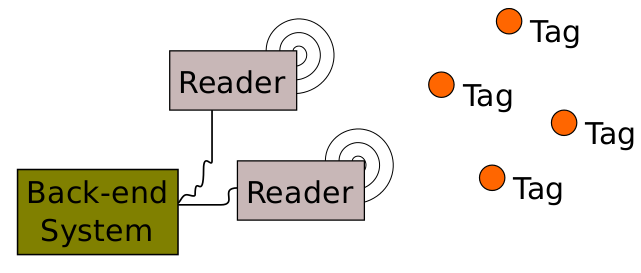
\includegraphics[width=4cm]{img/archRFID}
        \end{tabular}
\end{description}

\subsection{History}

\begin{itemize}
    \item 1930: First experimentations
    \item 1980: Commercialization
\end{itemize}


\subsection{Daily Life Example}

\begin{tabular}{m{6cm}m{6cm}}
	Basic RFID & Evolved RFID\\
		\begin{itemize}
    			\item Pet identification
    			\item Localisation
    			\item Book borrowing and inventories
		\end{itemize} &

	\begin{itemize}
			\item Building Access Control
			\item Payments
			\item Electronic documents
		\end{itemize}
\end{tabular}

	
\subsection{Tags Characteristics}
\begin{center}
    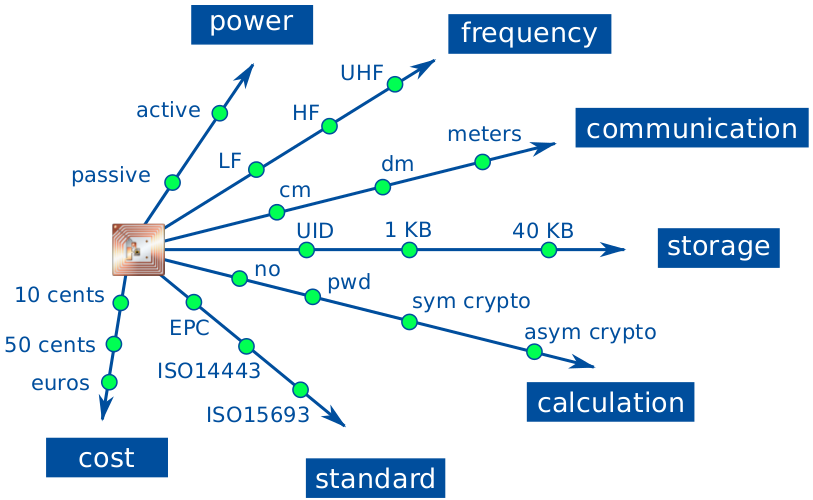
\includegraphics[width=9cm]{img/characRFID}
\end{center}

\subsubsection{Power Source}
\begin{itemize}
    \item \textbf{Passive}:  Tags don't have any internal energy source. They
    get energy from the reader's electromagnetic field.
\item \textbf{Active}:  Tags have a battery that is used both for internal
    calculations and transmission.
\item \textbf{Semi-Passive}:  Tags only have energy for the calculation.
\end{itemize}


\subsubsection{Frequency Bands}
\begin{center}
    \begin{tabular}{|c|c|c|}
        \hline
        & \textbf{Frequency} & \textbf{Range} \\
        \hline
        Low Frequency (ISO 18000 part 2) &  124\text{-}135 kHz & centimeters \\
        High Frequency (ISO 18000 part 3) &  13.56 MHz & decimeters \\
        Ultra-High Frequency (ISO 18000 part 6) & 860\text{-}960 MHz & meters \\
        \hline
    \end{tabular}
\end{center}

\begin{itemize}
    \item Skimming: With a stronger power and better antennas, a tag
        can be read at a greater distance (more than 1m for HF).
    \item Eavesdropping: Reader-to-tag channel (\textbf{forward}) can be
        generally read at a distance greater than tag-to-reader channel
        (\textbf{backward}). (True for \textsc{ISO-14443A}, but false
        for \textsc{ISO-14443B})
\end{itemize}

\subsubsection{Memory}
\begin{itemize}
    \item Tags have at least a few bits to store unique identifier
        \textbf{UID} (32 to 128bits) usually chosen by the manufacturer
        and cannot be changed by the user.
    \item \textbf{EEPROM}, additional memory, can be added: 1KB usually
        to 70KB for passport
\end{itemize}

\paragraph{Note :} Do not use \textbf{UID} for access control because
it can be simulated in a communication.

\subsubsection{Security}

\begin{description}
    \item[Tamper-resistance] A device is tamper-resistant if no adversary can
    get access to its protected memory by use of side-channel attacks.
    \item[Side-channel attack] An attack where the information is
        retrieved from physical implementation of a system. For example,
        (1)~Timing attack, (2)~physical attack, (3)~power analysis
        attacks, (4)~fault injection attacks, ...).
\end{description}

\paragraph{Computation Capabilities}:

\begin{tabular}{m{0.5cm}m{15cm}}
    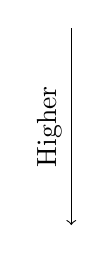
\begin{tikzpicture}
        \draw (0, 0) edge[<-] node[left] {\rotatebox{90}{Higher}} (0,
        2.5);
    \end{tikzpicture}
    &
\begin{enumerate}
    \item No computation capabilities, only memory
    \item Simple logic operation
    \item Symmetric cryptography (DES, AES) and microprocessor not
        necessarily required. $\Rightarrow$ LF and HF
    \item Asymmetric cryptographic with microprocessor.
        $\Rightarrow$ HF only currently
\end{enumerate}
\end{tabular}

\subsubsection{Object Name Service}
 The Object Name Service allows to discorver information about a product and related
 service. It allows for object (in this case tag) to communicate with device connected to 
 a network. Each tag own an EPC identifer.
%TODO slide 82 ONS

\paragraph{Near Field Communication (NFC)}
NFC is an extension of RFID, its main difference its that it offer
Peer-to-Peer connections between two (active) devices. NFC Data are exchanged
in a different format.


\subsection{Communication with Tag \textsc{ISO-7816} compliant}

\subsubsection{Memory}
    Internal structure composed of two type of files:
\begin{itemize}
    \item Dedicated File (\textbf{DF})
    \item Elementary File (\textbf{EF}) that can be identified in two subtypes
    \begin{description}
        \item[Internal] Store information used by the card for management and
        control purpose.
        \item[External] Store information used exclusively by the outside world
    \end{description}
    
    \paragraph{Data}
    Data inside an EF is stored in different formats:
    \begin{description}
        \item \textbf{data unit}:  Smallest set of bits which can be unambiguously
            referenced. Default value is 1 byte.
        \item \textbf{record}:  String of bytes which can be handled as a whole. Record
            can be referenced by an 8-bit identifier.
        \item \textbf{data object}:  Structure of information which consists of a tag, a
            length and a value.
    \end{description}
\end{itemize}

\paragraph{Note} The Master File (\textbf{MF}) is a special \textbf{DF}
and is the only mandatory file. Each application is stored in a distinct
\textbf{DF}.

\begin{center}
    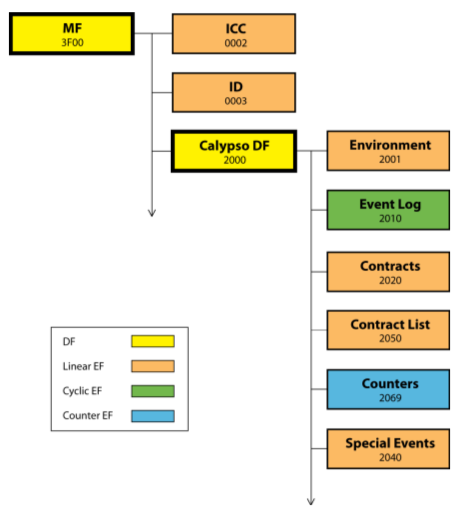
\includegraphics[width=6cm]{img/7816}
\end{center}

\subsubsection{APDU}
Application Protocol Data Unit : CLAss,INStruction,Param1,Param2,Length + Data
\begin{itemize}
	\item Class = Indicates the type of command (interindustry or proprietary)
	\item Instruction = Indicate the specific command (ex:write data)
	\item Param1-2 = Parameter used by the instruction (ex:file and offset)
	\item Length +data

\end{itemize}


\paragraph{Communication}
The protocol used to exchange data is the Application Protocol Data Unit.


